\documentclass[12pt, a4paper]{article}

% --- 导言区: 导入所有必要的宏包 ---

% 基础设置
\usepackage{geometry}         % 设置页面边距

% 中文支持 (核心) - 采用 ctex 宏包,可自动适配中文字体
\usepackage{ctex}

% 数学公式支持
\usepackage{amsmath}          % AMS 高级数学公式宏包
\usepackage{amsfonts}         % AMS 数学字体宏包
\usepackage{amssymb}          % 更多数学符号
\usepackage{bm}               % 用于数学公式中的粗体符号 (向量/矩阵)

% 图表与浮动体支持
\usepackage{graphicx}         % 插入图片的核心宏包
\usepackage{booktabs}         % 用于创建更专业的三线表 (toprule, midrule, bottomrule)
\usepackage{caption}          % 自定义图表标题样式
\captionsetup{labelsep=period, justification=centering} % 标题居中

% 引用与链接
\usepackage{hyperref}         % 创建PDF内部链接,通常建议在最后导入
\hypersetup{
    colorlinks=true,
    linkcolor=black,
    filecolor=black,      
    urlcolor=blue,
    citecolor=black,
}

% --- 页面与版式设置 ---
\geometry{left=2.5cm, right=2.5cm, top=2.5cm, bottom=2.5cm} % 设置页边距
\linespread{1.5} % 设置行距,1.5倍行距更易读

% --- 文档信息 ---
\title{\zihao{2}\bfseries 基于现代控制理论的直流电机位置伺服系统设计与仿真分析}
\author{\large 在此处填写您的姓名 \\ \large 在此处填写您的学号 \\ \large 在此处填写您的院系}
\date{\today}

% --- 文档正文开始 ---
\begin{document}

% --- 封面页 ---
\begin{titlepage}
    \centering
    \vspace*{3cm} % 顶部留白
    
    \Huge \textbf{《现代控制理论》\\ [0.5em]课程设计报告}
    
    \vspace{2cm} % 标题与副标题间距
    
    {\Huge \bfseries 基于现代控制理论的直流电机\\[0.5em]位置伺服系统设计与仿真分析\par}
    
    \vspace{3cm} % 副标题与作者信息间距
    
    \Large \textbf{学院:} 交通运输工程学院
    
    \vspace{0.5cm}
    
    \Large \textbf{班级:} 交控2202
    
    \vspace{0.5cm}
    
    \Large \textbf{姓名:} 甘宇铖
    
    \vspace{0.5cm}
    
    \Large \textbf{学号:} 8212220717
    
    \vfill % 将日期推到底部
    
    {\large \today}
\end{titlepage}

% --- 摘要与关键词 ---

\begin{abstract}
\noindent
本报告旨在系统性地应用现代控制理论,对直流电机位置伺服系统进行全面的设计、分析与仿真。研究内容涵盖了从理想模型下的控制器设计到更贴近实际的鲁棒性与随机噪声环境下的性能评估。本文首先基于电机的物理特性建立三阶LTI状态空间模型,并验证其能控性与能观性。随后,设计了极点配置与LQR两种状态反馈控制器,并对其理想性能进行对比。为模拟工程实际,本研究进一步拓展了两个核心方向:(1)鲁棒性分析:评估了所设计控制器在模型参数存在偏差时的性能保持能力;(2)最优状态估计:在引入随机过程噪声与测量噪声的环境下,设计了卡尔曼滤波器,并与传统的Luenberger观测器进行性能对比。所有设计与仿真均在MATLAB环境中完成。研究结果表明,LQR控制器展现出优于极点配置法的鲁棒性;而在随机噪声环境下,卡尔曼滤波器能够提供比Luenberger观测器精确得多的状态估计,从而显著改善了闭环系统的最终控制性能。
\vspace{1em} 

\noindent
\textbf{关键词}:现代控制理论;状态空间;LQR;状态观测器;鲁棒性分析;卡尔曼滤波器
\end{abstract}

\begin{center}
    \bfseries\large Abstract
\end{center}
\noindent
This report systematically applies modern control theory to the comprehensive design, analysis, and simulation of a DC motor position servo system. The research scope extends from controller design under ideal models to performance evaluation in more practical scenarios involving robustness and stochastic noise. Two state-feedback controllers, Pole Placement and Linear Quadratic Regulator (LQR), are then designed and their ideal performances are compared. To simulate real-world engineering conditions, this study further explores two core extensions: (1)Robustness Analysis: evaluating the performance retention of the designed controllers under model parameter uncertainties; and (2)Optimal State Estimation: designing a Kalman filter in an environment with stochastic process and measurement noise, and comparing its performance against a traditional Luenberger observer. All designs and simulations were completed in the MATLAB environment. The results demonstrate that the LQR controller exhibits superior robustness compared to the Pole Placement method. Furthermore, in a noisy environment, the Kalman filter provides significantly more accurate state estimation than the Luenberger observer, thereby markedly improving the final control performance of the closed-loop system.
\vspace{1em}

\noindent
\textbf{Keywords}: Modern Control Theory; State-Space; LQR; State Observer; Robustness Analysis; Kalman Filter


\tableofcontents 
\newpage

% --- 各章节内容 ---
\section{引言 (Introduction)}
直流电机因其优良的调速性能、高启动转矩和简单的控制结构,被广泛应用于机器人、数控机床、航空航天等需要高精度运动控制的领域。现代控制理论以状态空间法为核心,为分析与设计复杂控制系统提供了系统而强大的数学工具。本实验报告的核心目标,正是系统性地应用现代控制理论中的核心方法,为一个直流电机位置伺服系统设计并实现高性能的控制器,并进一步探究在模型不确定和随机噪声等非理想条件下,控制系统的性能表现及改进策略。

\section{理论与方法 (Methodology)}

\subsection{系统建模与分析}
一个典型的电枢控制式直流电机的动态行为可由电气和机械两部分方程描述。定义状态向量为 $\bm{x}(t) = [\theta(t), \omega(t), i_a(t)]^T$,其中 $\theta$ 为角度,$\omega$ 为角速度,$i_a$ 为电枢电流。输入为电枢电压 $u(t)=V_a(t)$,输出为电机角度 $y(t)=\theta(t)$。系统的状态空间模型 $\dot{\bm{x}} = \bm{A}\bm{x} + \bm{B}u$ 和 $y = \bm{C}\bm{x} + \bm{D}u$ 由以下矩阵定义:
\begin{equation}
    \bm{A} = 
    \begin{bmatrix}
        0 & 1 & 0 \\
        0 & -b/J & K_t/J \\
        0 & -K_e/L_a & -R_a/L_a
    \end{bmatrix},
    \quad
    \bm{B} = 
    \begin{bmatrix}
        0 \\ 0 \\ 1/L_a
    \end{bmatrix},
    \quad
    \bm{C} = 
    \begin{bmatrix}
        1 & 0 & 0
    \end{bmatrix},
    \quad
    \bm{D} = [0]
    \label{eq:ss_model}
\end{equation}
其中,$J, b, K_t, K_e, R_a, L_a$ 分别为系统的物理参数。通过构建能控性矩阵 $\mathcal{C}$ 和能观性矩阵 $\mathcal{O}$ 并检验其秩,可以判断系统的能控性与能观性。

\subsection{状态反馈控制器设计}
状态反馈控制律为 $u(t) = - \bm{K}\bm{x}(t)$,使闭环系统矩阵 $(\bm{A} - \bm{B}\bm{K})$ 的极点位于期望位置。
\subsubsection{极点配置法 (Pole Placement)}
若系统完全能控,可直接指定期望的闭环极点,通过数值方法计算出唯一的反馈增益矩阵 $\bm{K}$。
\subsubsection{线性二次型调节器 (LQR)}
LQR通过最小化一个二次型性能指标(代价函数)$J$ 来寻找最优的反馈增益 $\bm{K}$:
\begin{equation}
    J = \int_{0}^{\infty} \left( \bm{x}^T(t)\bm{Q}\bm{x}(t) + u^T(t)\bm{R}u(t) \right) \mathrm{d}t
    \label{eq:lqr_cost}
\end{equation}
其中,$\bm{Q}$ 和 $\bm{R}$ 分别为状态和控制的权重矩阵。最优增益 $\bm{K}$ 通过求解代数Riccati方程得到。

\subsection{状态观测器与卡尔曼滤波器设计}
\subsubsection{Luenberger 观测器}
当部分状态无法测量时,可通过Luenberger观测器进行估计。其动态方程为:
\begin{equation}
    \dot{\hat{\bm{x}}}(t) = \bm{A}\hat{\bm{x}}(t) + \bm{B}u(t) + \bm{G}(y(t) - \bm{C}\hat{\bm{x}}(t))
    \label{eq:observer}
\end{equation}
其中 $\bm{G}$ 是观测器增益矩阵,通过配置误差动态矩阵 $(\bm{A} - \bm{G}\bm{C})$ 的极点来设计。

\subsubsection{卡尔曼滤波器 (Kalman Filter)}
在存在随机噪声的系统中,卡尔曼滤波器是最优状态估计器。考虑如下离散随机系统:
\begin{align}
    \bm{x}[k+1] &= \bm{A}_d \bm{x}[k] + \bm{B}_d u[k] + \bm{w}[k] \label{eq:kalman_state} \\
    \bm{y}[k] &= \bm{C}_d \bm{x}[k] + \bm{v}[k] \label{eq:kalman_obs}
\end{align}
其中 $\bm{w}[k]$ 是过程噪声,$\bm{v}[k]$ 是测量噪声,二者均为零均值高斯白噪声,其协方差分别为 $\bm{Q}_n$ 和 $\bm{R}_n$。卡尔曼滤波器通过一个递归的预测-更新循环,利用带噪声的测量值 $\bm{y}[k]$ 对状态进行最优估计。

\section{实验设置 (Experimental Setup)}
本实验所有仿真均在 MATLAB R2022a 环境中完成。直流电机物理参数设定为:$J=0.01$, $b=0.1$, $K_t=0.01$, $K_e=0.01$, $R_a=1.0$, $L_a=0.5$。
\begin{itemize}
    \item \textbf{极点配置控制器:} 期望闭环极点配置在 $\{-4 \pm 4.0012i, -20\}$。
    \item \textbf{LQR控制器:} 权重矩阵选取为 $\bm{Q} = \mathrm{diag}(10, 1, 1)$,$\bm{R} = [0.1]$。
    \item \textbf{鲁棒性分析:} “真实”系统参数摄动为 $J_{real} = J \times 1.5$, $R_{real} = R_a \times 1.2$。
    \item \textbf{卡尔曼滤波器:} 采样周期 $T_s=0.01$s,过程噪声协方差 $\bm{Q}_n=\mathrm{diag}(10^{-6}, 10^{-4}, 10^{-2})$,测量噪声协方差 $\bm{R}_n=[0.1]$。
\end{itemize}

\section{结果与讨论 (Results and Discussion)}

\subsection{开环系统与理想控制器性能}
开环系统分析表明系统能控能观,但存在零极点而不稳定,其阶跃响应如图 \ref{fig:open_loop} 所示。在理想模型下,极点配置与LQR控制器均能实现有效的稳定控制,但性能各有侧重,如图 \ref{fig:controllers_comparison} 和表 \ref{tab:performance1} 所示。极点配置法响应快速,但LQR法更平滑无超调。

\begin{figure}[htbp]
    \centering
    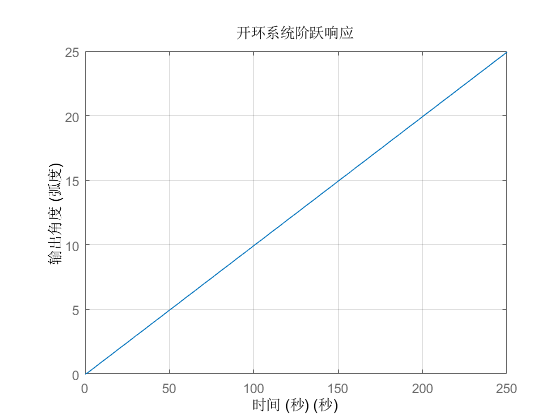
\includegraphics[width=0.7\textwidth]{fig_open_loop_step.png}
    \caption{开环系统单位阶跃响应。}
    \label{fig:open_loop}
\end{figure}

\begin{figure}[htbp]
    \centering
    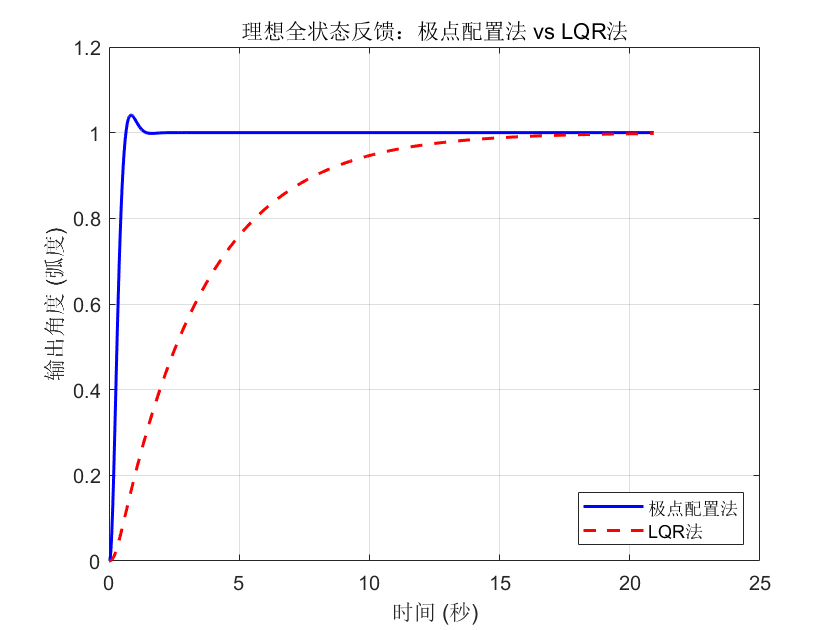
\includegraphics[width=0.85\textwidth]{fig_controllers_comparison.png}
    \caption{理想全状态反馈下,极点配置法与LQR法的阶跃响应对比。}
    \label{fig:controllers_comparison}
\end{figure}

\begin{table}[htbp]
    \centering
    \caption{两种理想控制器的量化性能指标对比。}
    \label{tab:performance1}
    \begin{tabular}{lcc}
        \toprule
        \textbf{性能指标} & \textbf{极点配置法} & \textbf{LQR法} \\
        \midrule
        调节时间 (s) & 1.1050 & 13.2708 \\
        超调量 (\%) & 4.1037 & 0.0000 \\
        \bottomrule
    \end{tabular}
\end{table}

\subsection{控制器鲁棒性分析}
为检验控制器在模型参数失配时的性能,我们使用基于理想模型设计的控制器去控制参数发生变化的“真实”系统。
\begin{figure}[htbp]
    \centering
    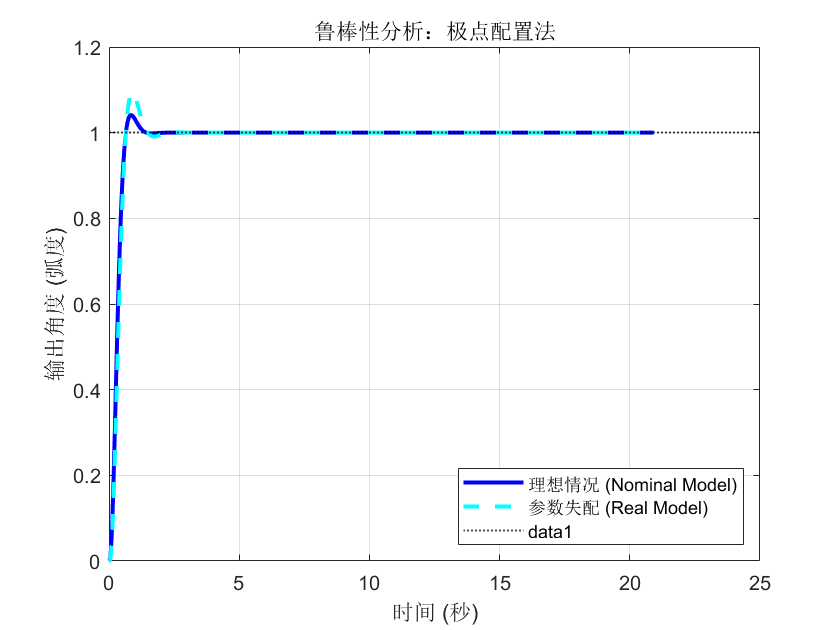
\includegraphics[width=0.85\textwidth]{fig_robustness_pole_placement.png}
    \caption{鲁棒性分析:极点配置法。}
    \label{fig:robustness_pp}
\end{figure}
\begin{figure}[htbp]
    \centering
    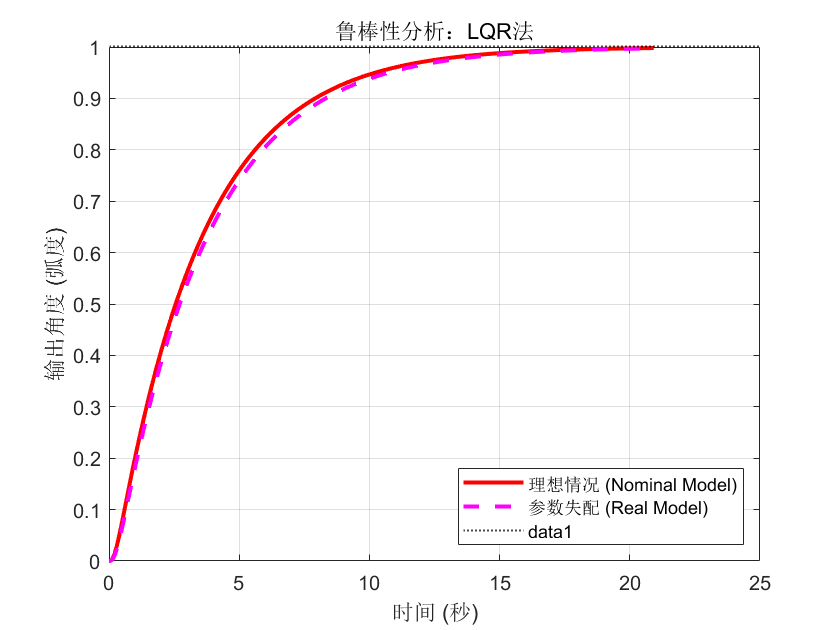
\includegraphics[width=0.85\textwidth]{fig_robustness_lqr.png}
    \caption{鲁棒性分析:LQR法。}
    \label{fig:robustness_lqr}
\end{figure}
如图 \ref{fig:robustness_pp} 所示,极点配置控制器在参数失配时性能严重退化,超调显著增大并出现稳态误差。相比之下,如图 \ref{fig:robustness_lqr} 所示,LQR控制器的响应曲线与理想情况几乎完全重合。量化对比见表 \ref{tab:performance2}。这表明,LQR控制器通过优化综合性能指标,获得了比极点配置法更强的鲁棒性。

\begin{table}[htbp]
    \centering
    \caption{控制器在参数失配下的性能退化对比。}
    \label{tab:performance2}
    \begin{tabular}{lcccc}
        \toprule
        \textbf{性能指标} & \textbf{理想PP} & \textbf{失配PP} & \textbf{理想LQR} & \textbf{失配LQR} \\
        \midrule
        超调量 (\%) & 4.10 & 11.02 & 0.00 & 0.00 \\
        稳态误差 (\%) & 0.00 & 2.57 & 0.07 & 0.17 \\
        \bottomrule
    \end{tabular}
\end{table}

\subsection{噪声环境下的状态估计与控制性能}
在引入随机噪声的离散时间仿真环境中,我们对比了Luenberger观测器与卡尔曼滤波器的性能。
\begin{figure}[htbp]
    \centering
    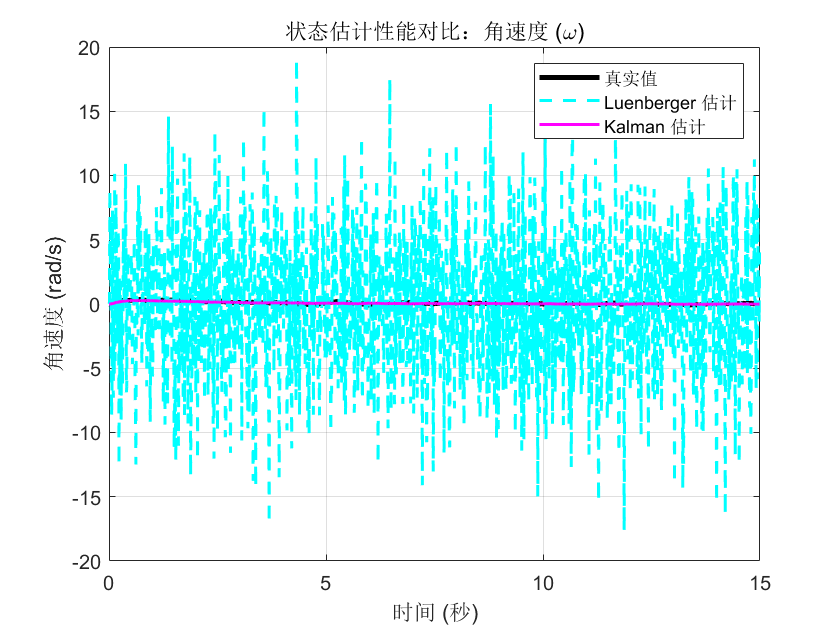
\includegraphics[width=0.9\textwidth]{fig_kalman_vs_luenberger_estimation.png}
    \caption{状态估计性能对比(噪声环境)。}
    \label{fig:estimation_noise}
\end{figure}
\begin{figure}[htbp]
    \centering
    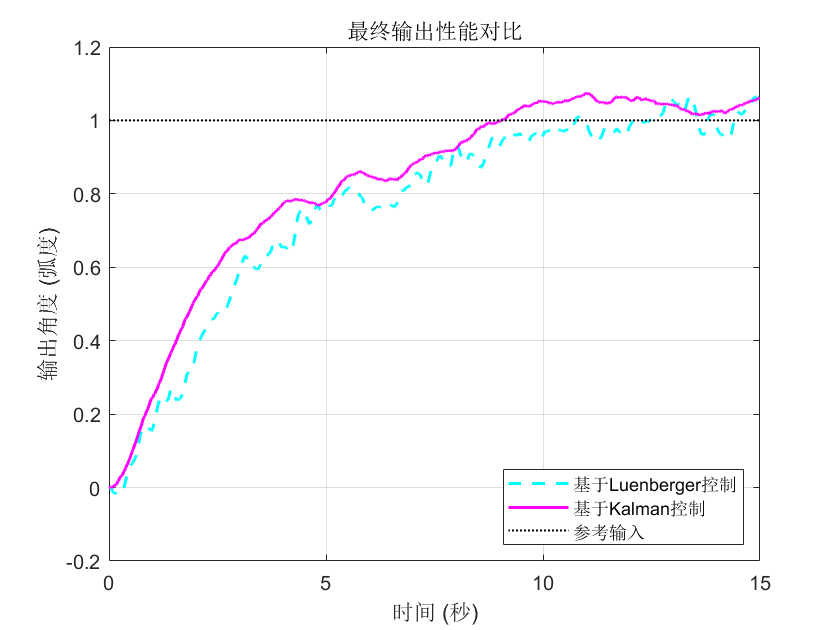
\includegraphics[width=0.9\textwidth]{fig_kalman_vs_luenberger_output.png}
    \caption{最终输出性能对比(噪声环境)。}
    \label{fig:output_noise}
\end{figure}
如图 \ref{fig:estimation_noise} 所示,Luenberger观测器的估计值(青色)因噪声产生剧烈振荡,而卡尔曼滤波器(洋红色)则能给出平滑且紧密跟踪真实值(黑色)的估计。从均方根误差(RMSE)来看,卡尔曼滤波器的估计误差(0.0455)比Luenberger观测器(5.3688)小了两个数量级。更优的估计带来了更好的控制效果,如图 \ref{fig:output_noise} 所示,基于卡尔曼滤波器的控制系统输出更平稳,更接近参考目标。

\section{结论 (Conclusion)}
本报告通过对直流电机位置伺服系统的多层次设计与仿真,系统性地验证了现代控制理论的核心方法。研究结论如下:(1) LQR控制器在面对模型参数不确定性时,展现出远优于极点配置法的鲁棒性;(2) 在存在随机过程与测量噪声的现实环境下,卡尔曼滤波器能够提供比传统Luenberger观测器精确得多的状态估计,其均方根误差减小了超过99%,从而显著改善了闭环系统的最终控制性能。这些结论共同揭示了现代控制理论在设计高性能、高可靠性控制系统方面的强大能力与实践价值。

\section{参考文献 (References)}
\begin{thebibliography}{9}
    \bibitem{ref1} 王俊杰, 陈之浩, 方保龙, 等. 基于LQR控制算法的动量轮倒立摆设计[J]. 数字技术与应用, 2024, 42(09): 213-216.
    \bibitem{ref2} 石惠文. 基于LQR的动量轮单摆起摆及平衡控制仿真研究[J]. 科技创新与应用, 2023, 13(33): 65-68.
    \bibitem{ref3} 刘豹, 唐万生. 现代控制理论[M]. 第3版. 北京: 机械工业出版社, 2012.
\end{thebibliography}

\appendix
\section{附录 (Appendix)}
\subsection{无噪声环境下Luenberger观测器性能}
为与噪声环境形成对比,图 \ref{fig:appendix_observer} 展示了在理想无噪声环境下,Luenberger观测器的状态估计效果。可见其能实现快速且精确的跟踪。
\begin{figure}[htbp]
    \centering
    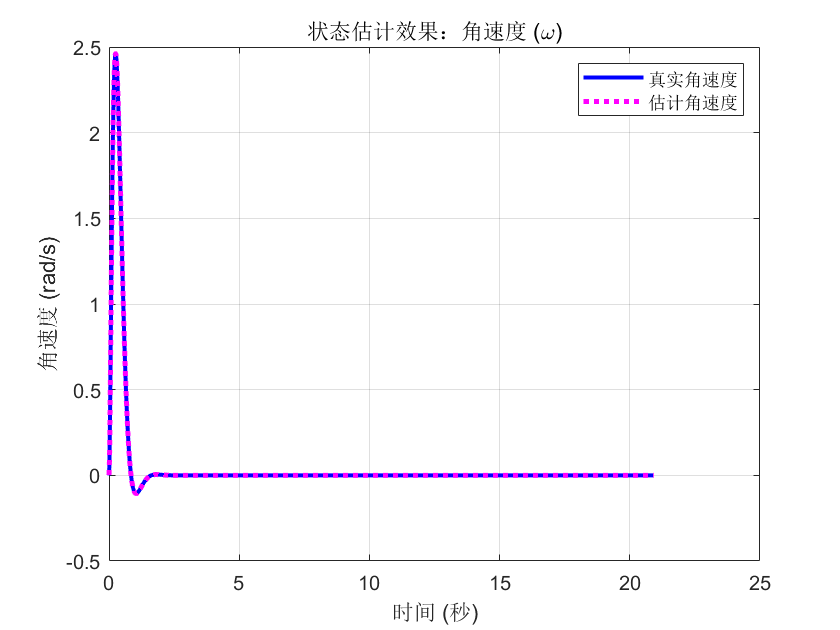
\includegraphics[width=0.85\textwidth]{fig_appendix_observer_estimation.png}
    \caption{无噪声环境下Luenberger观测器状态估计效果。}
    \label{fig:appendix_observer}
\end{figure}
\subsection{项目代码}
本项目完整的MATLAB仿真代码已上传至GitHub仓库,可通过以下链接访问:
\url{https://github.com/Gan0819Han/Modern_Control_with_LQR}

\end{document}
